\documentclass[aspectratio=169]{beamer}

% Define big arrow down
\newcommand{\xdownarrow}[1]{%
  {\left\downarrow\vbox to #1{}\right.\kern-\nulldelimiterspace}
}

% Packages used
\usepackage{xcolor,ulem}
\usepackage{listings}

% Title/author info
\title{Propagating Uncertainty Information through Gray-Box Multiobjective Optimization Problems}
\subtitle{Work (no longer) in Progress}
\author{Tyler Chang}
\institute{Siemens EDA (formerly Argonne National Laboratory)}
\date{Dagstuhl Seminar 26041, Jan 2026}

% Slides start here
\begin{document}

% Titleslide
\frame{\titlepage}

% FRAME: overview
% No TOC uncomment below:
% \begin{frame}
%   \frametitle{Outlines}
%   \tableofcontents
% \end{frame}

% ========================================
% main slides come here
% ========================================

\section{Introduction}

\begin{frame}\frametitle{Multiobjective ``Simulation'' Optimization Problems}
\begin{columns}
  \begin{column}{0.5\textwidth}
    \begin{center}
    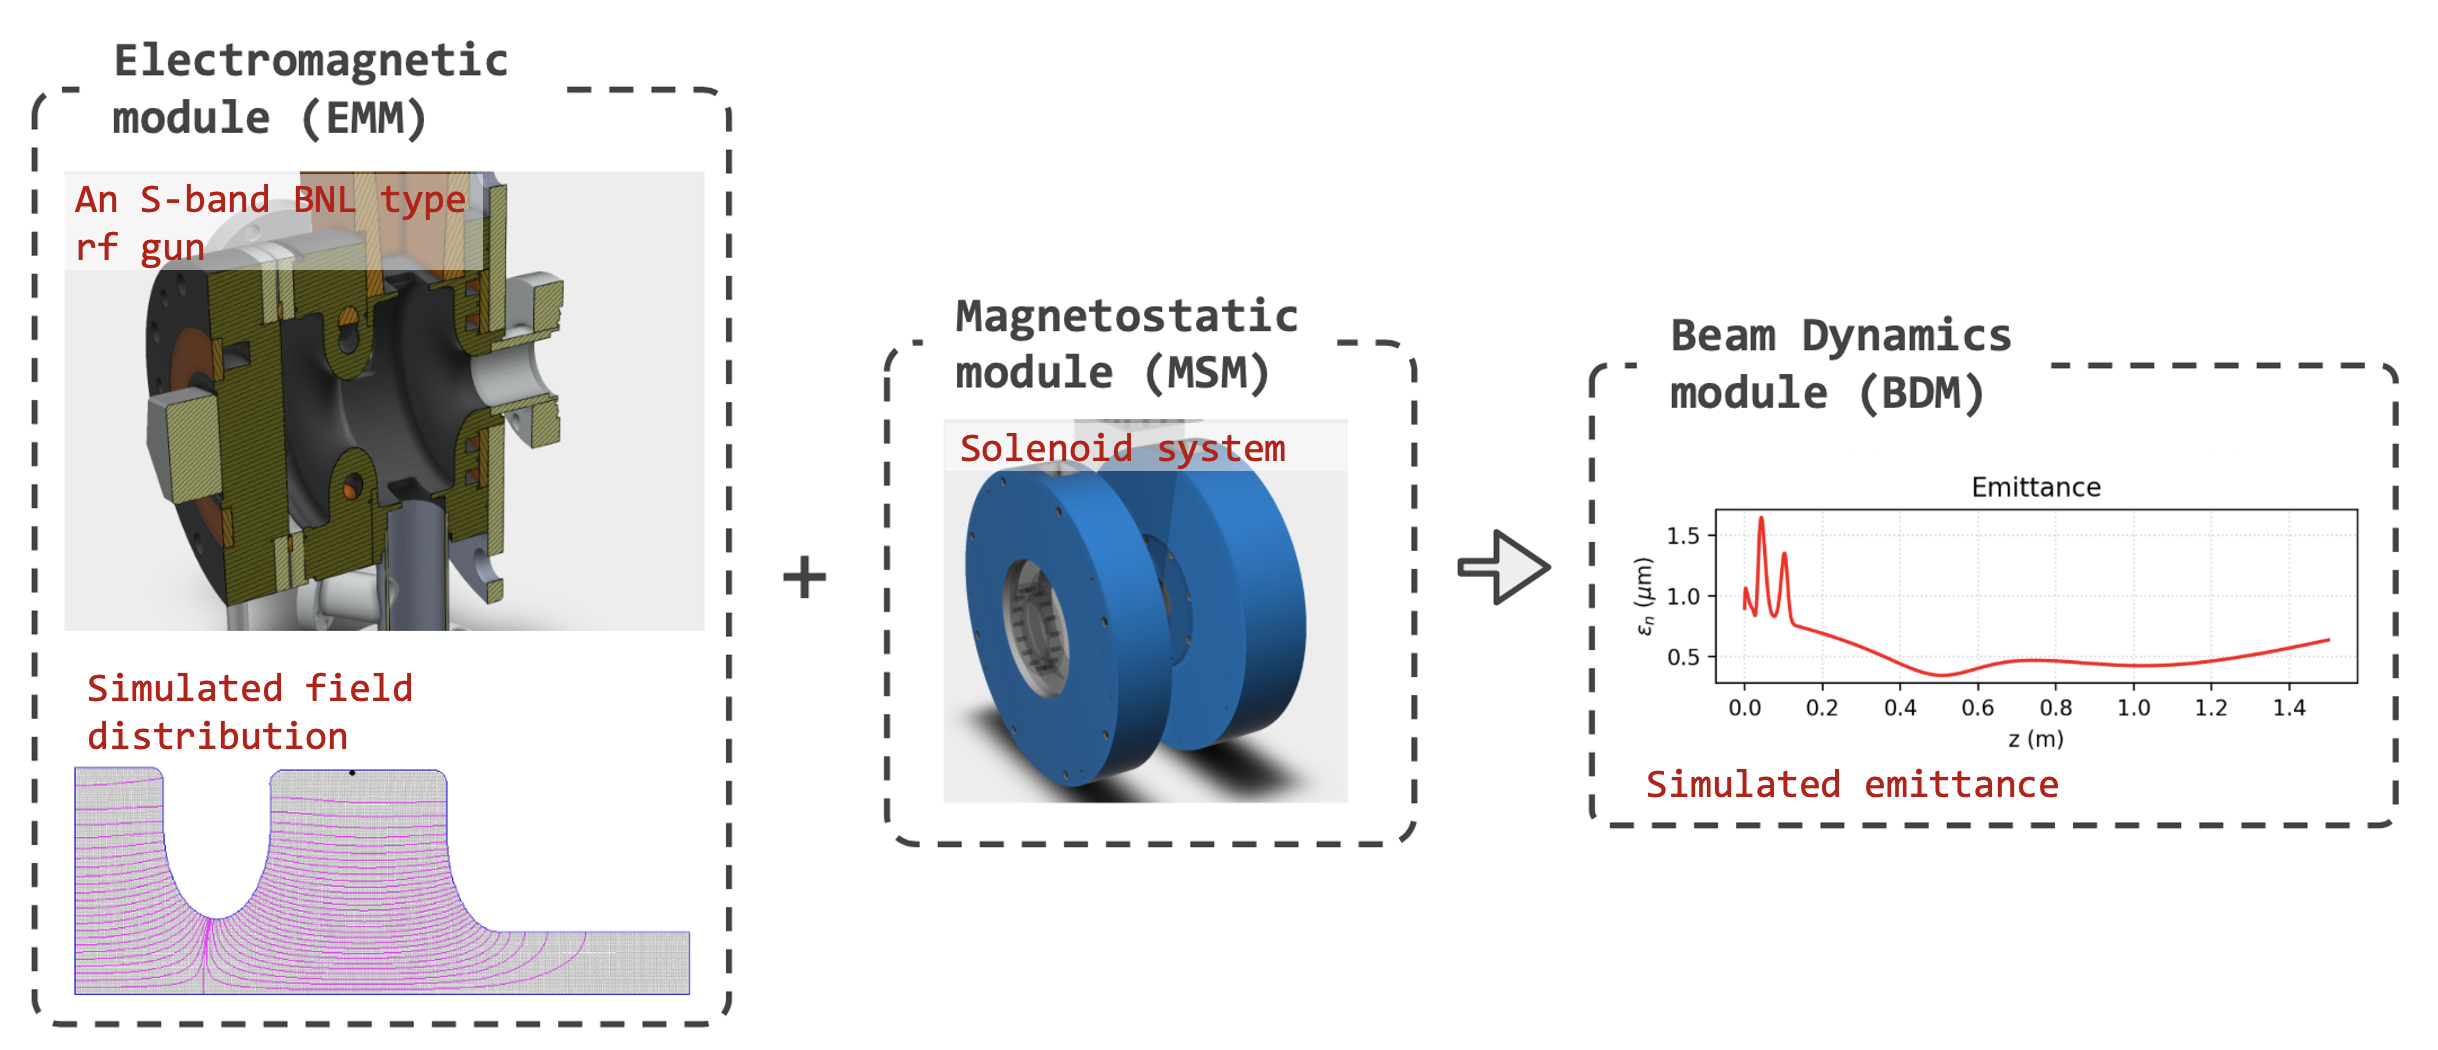
\includegraphics[width=0.6\textwidth]{../2023WSC/setup2.png}\\
    Tuning geometry of electron beam RF gun cavity (Linear accelerator) via
    multi-physics simulations
    \end{center}
  \end{column}
  \begin{column}{0.5\textwidth}
    \begin{center}
    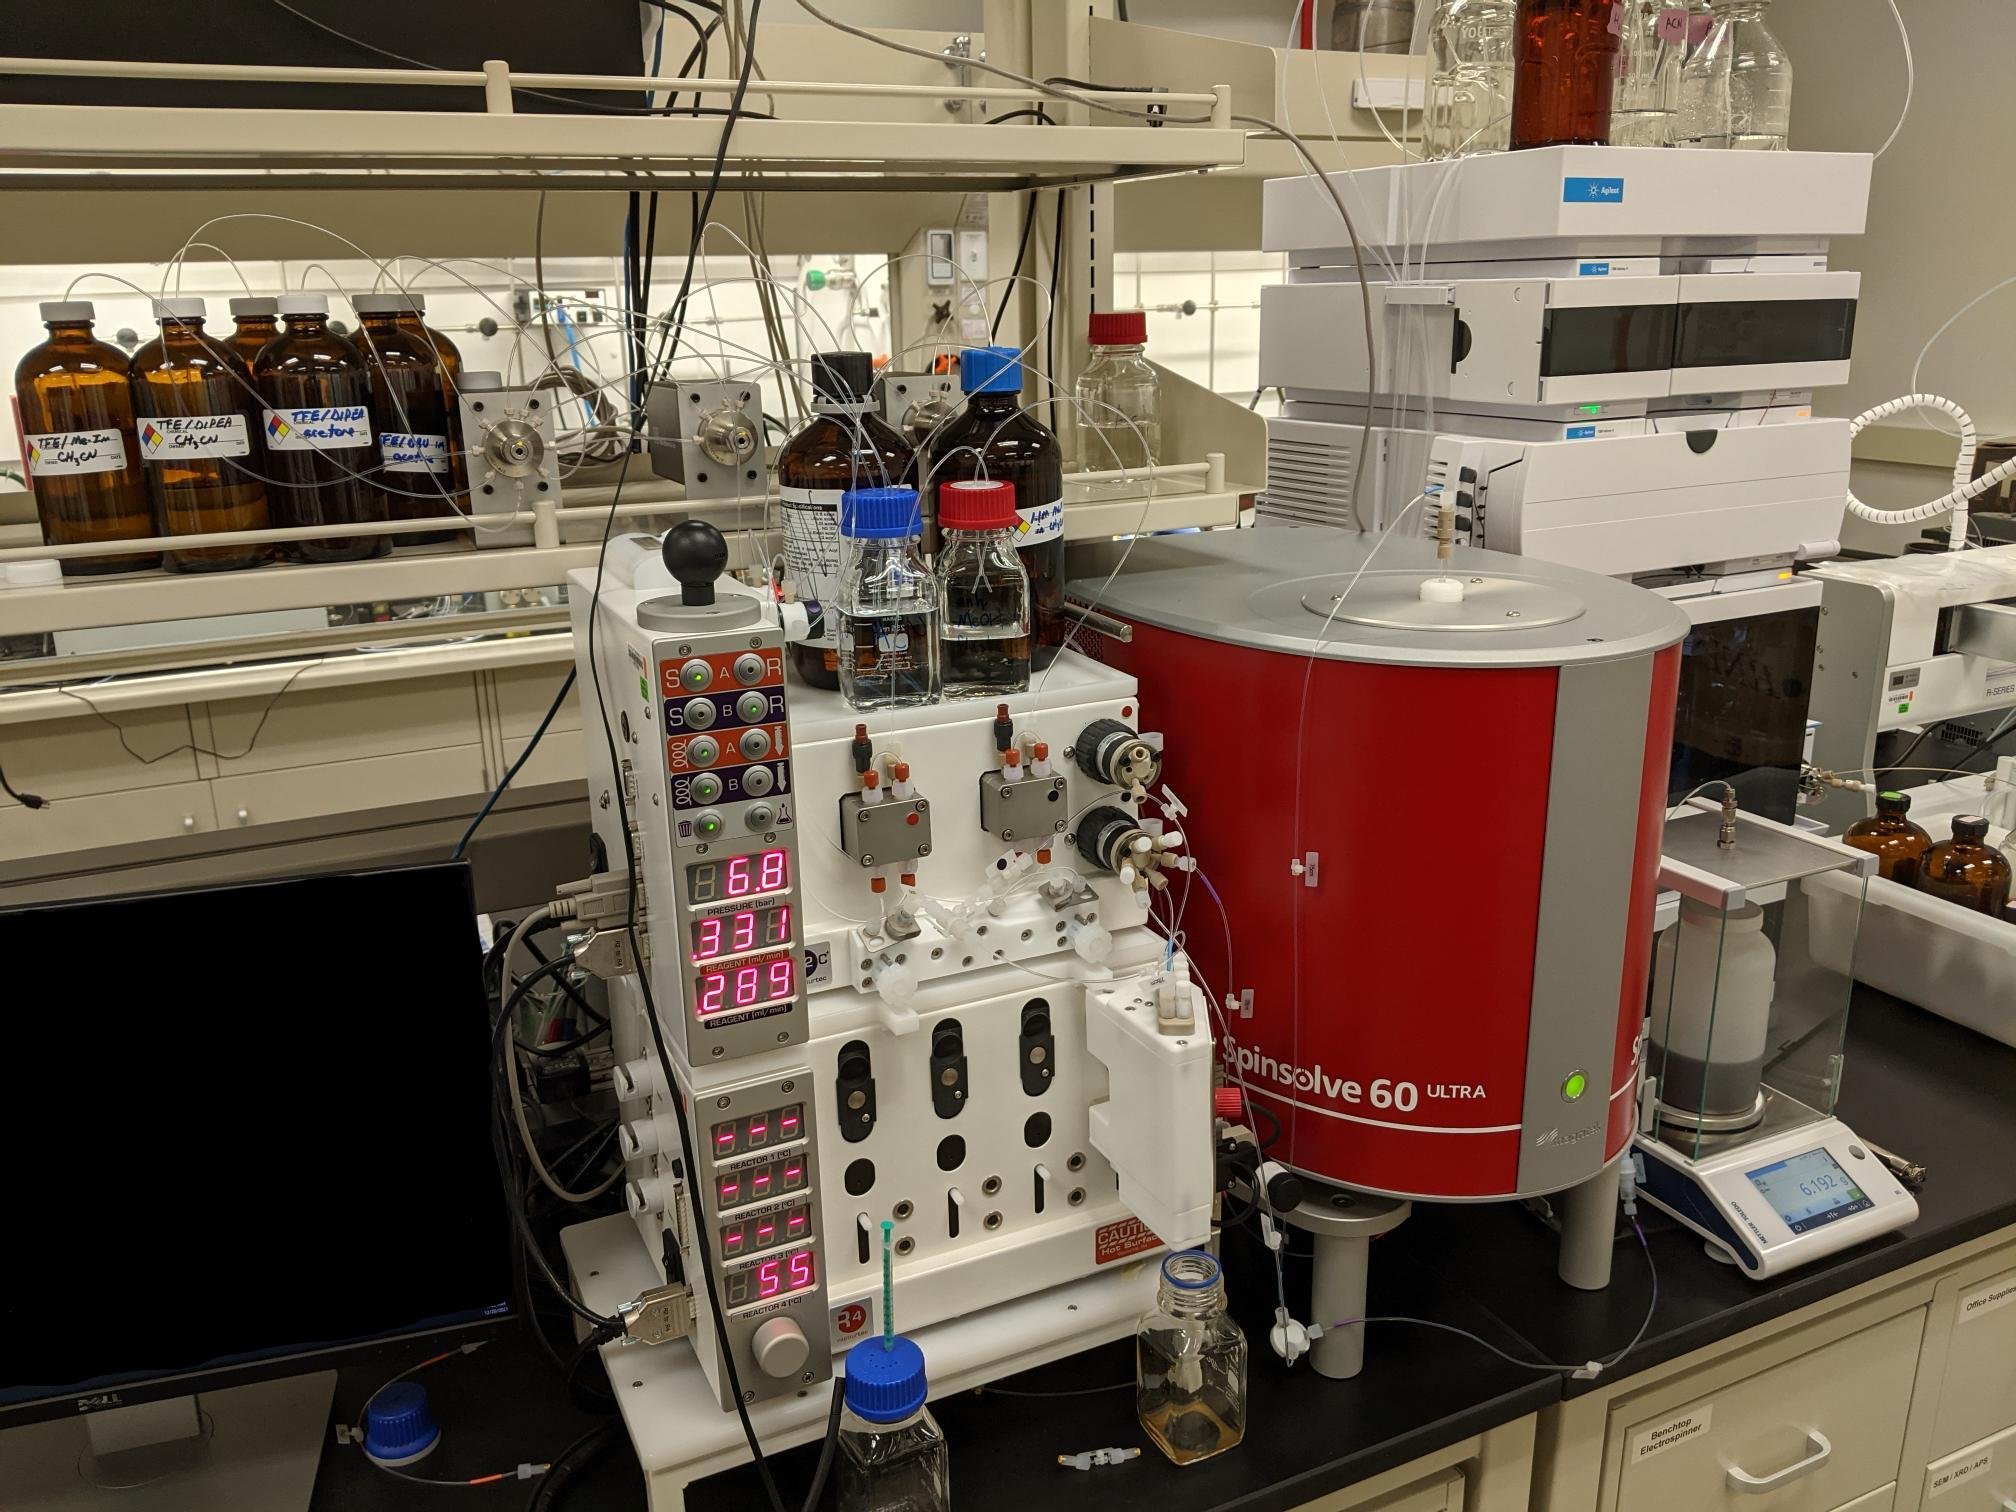
\includegraphics[width=0.4\textwidth]{../img/probs/cfr-nmr-setup.jpg}\\
    Automated continuous flow reactor settings for material manufacturing
    \end{center}
  \end{column}
\end{columns}
\begin{columns}
  \begin{column}{0.5\textwidth}
    \begin{center}
    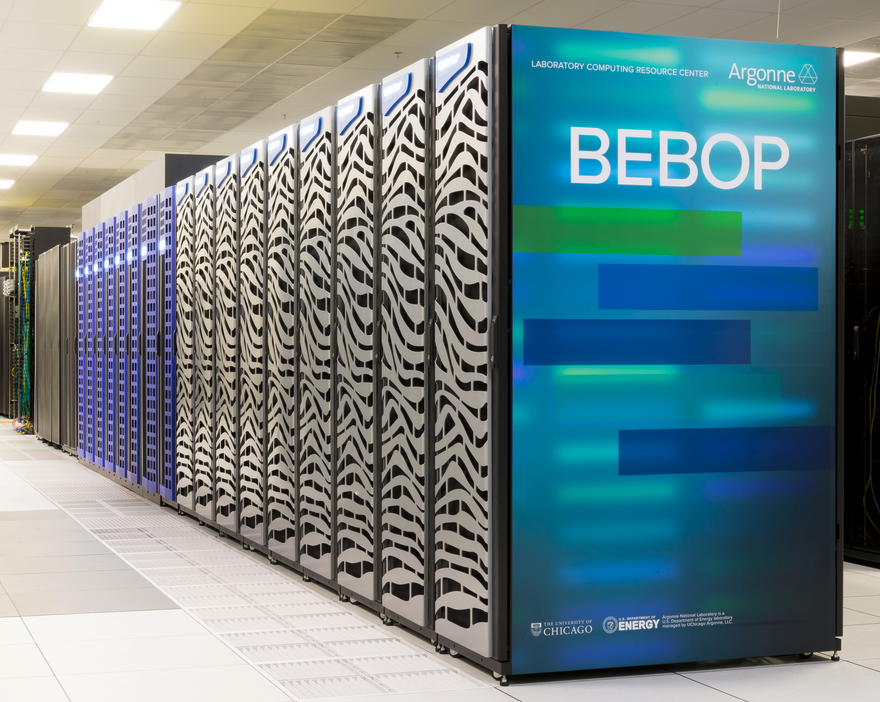
\includegraphics[width=0.35\textwidth]{../img/probs/anl-bebop.png}\\
    Autotuning (performance optimization) of HPC system libraries\\
    \end{center}
  \end{column}
  \begin{column}{0.5\textwidth}
    \begin{center}
    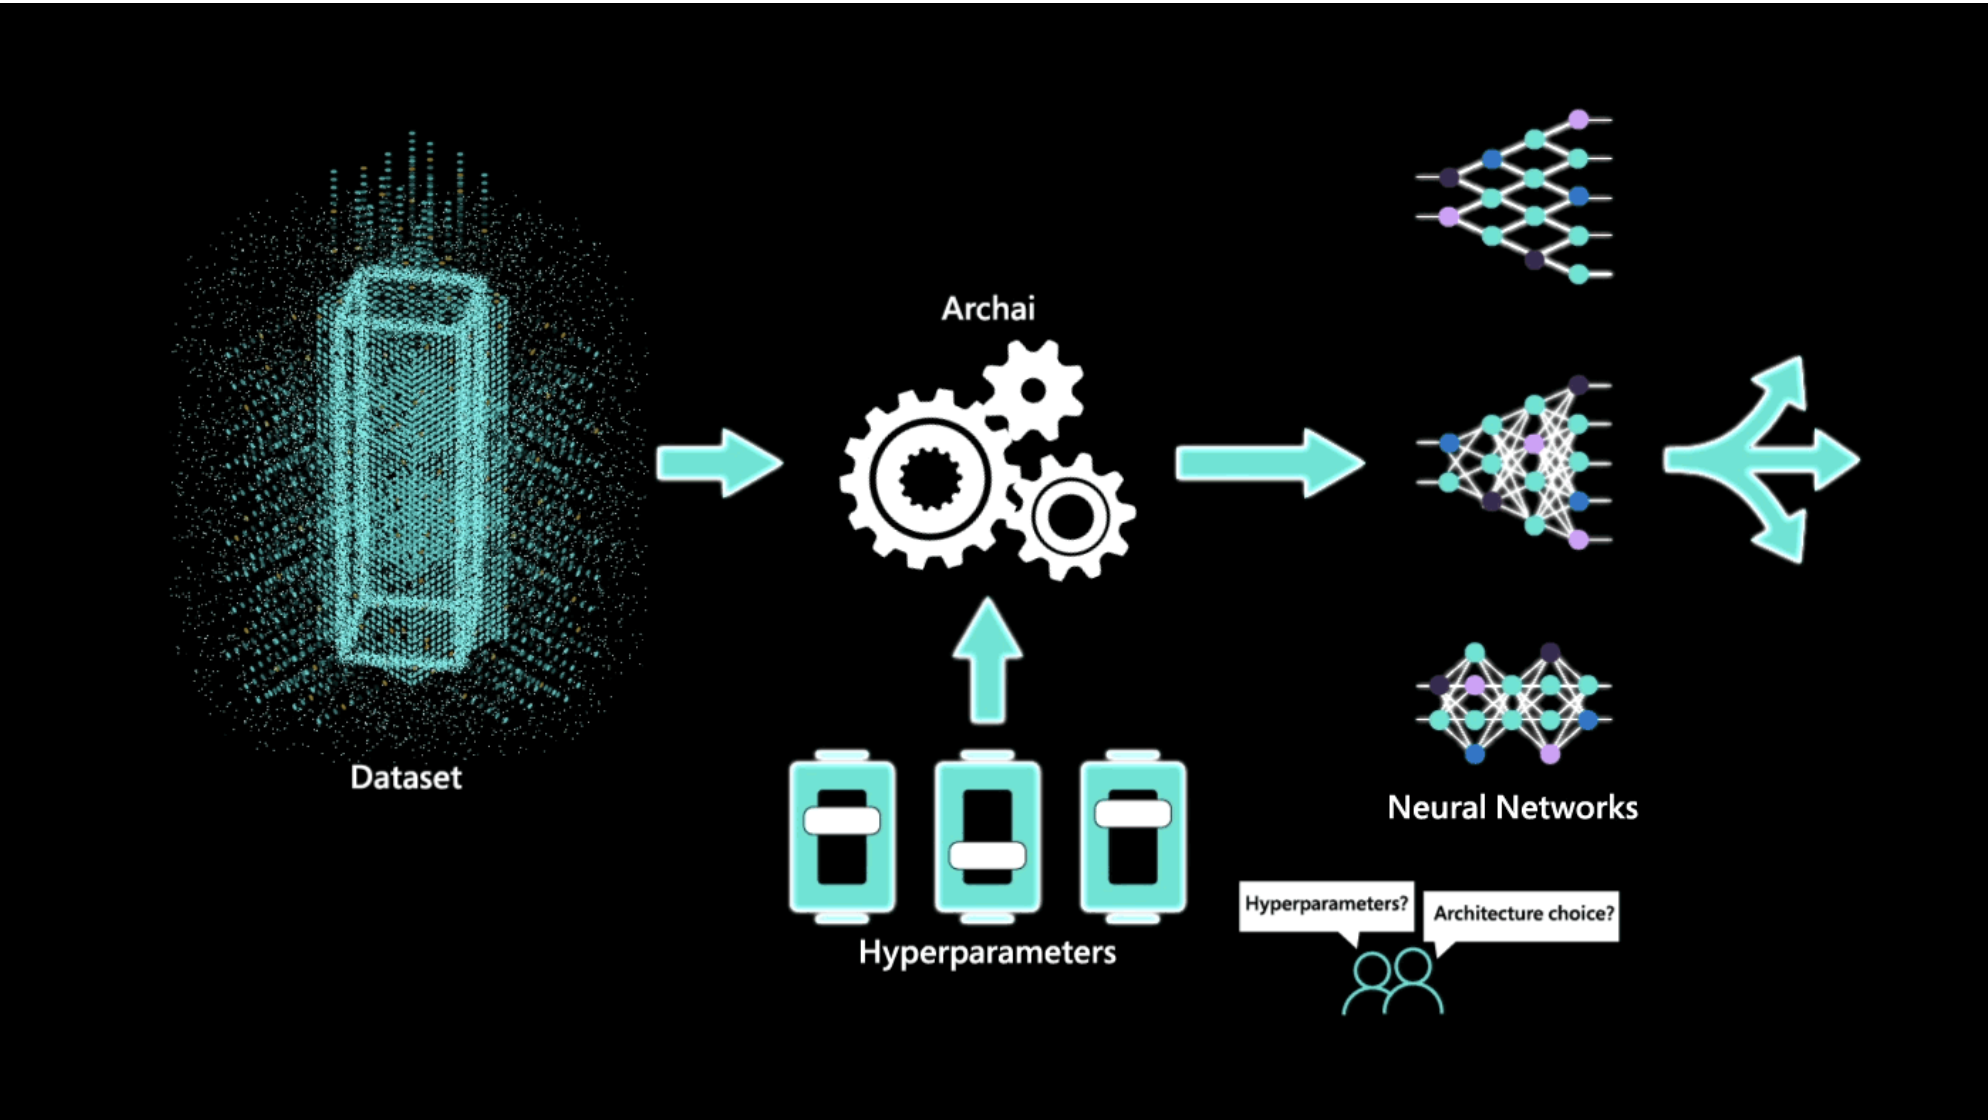
\includegraphics[width=0.5\textwidth]{../img/probs/microsoft-nas.png}\\
    Neural Architecture Search (image credit from Microsoft press release)
    \end{center}
  \end{column}
\end{columns}
\end{frame}

\begin{frame}\frametitle{Multi-layered ``Gray Box''}
\begin{center}
    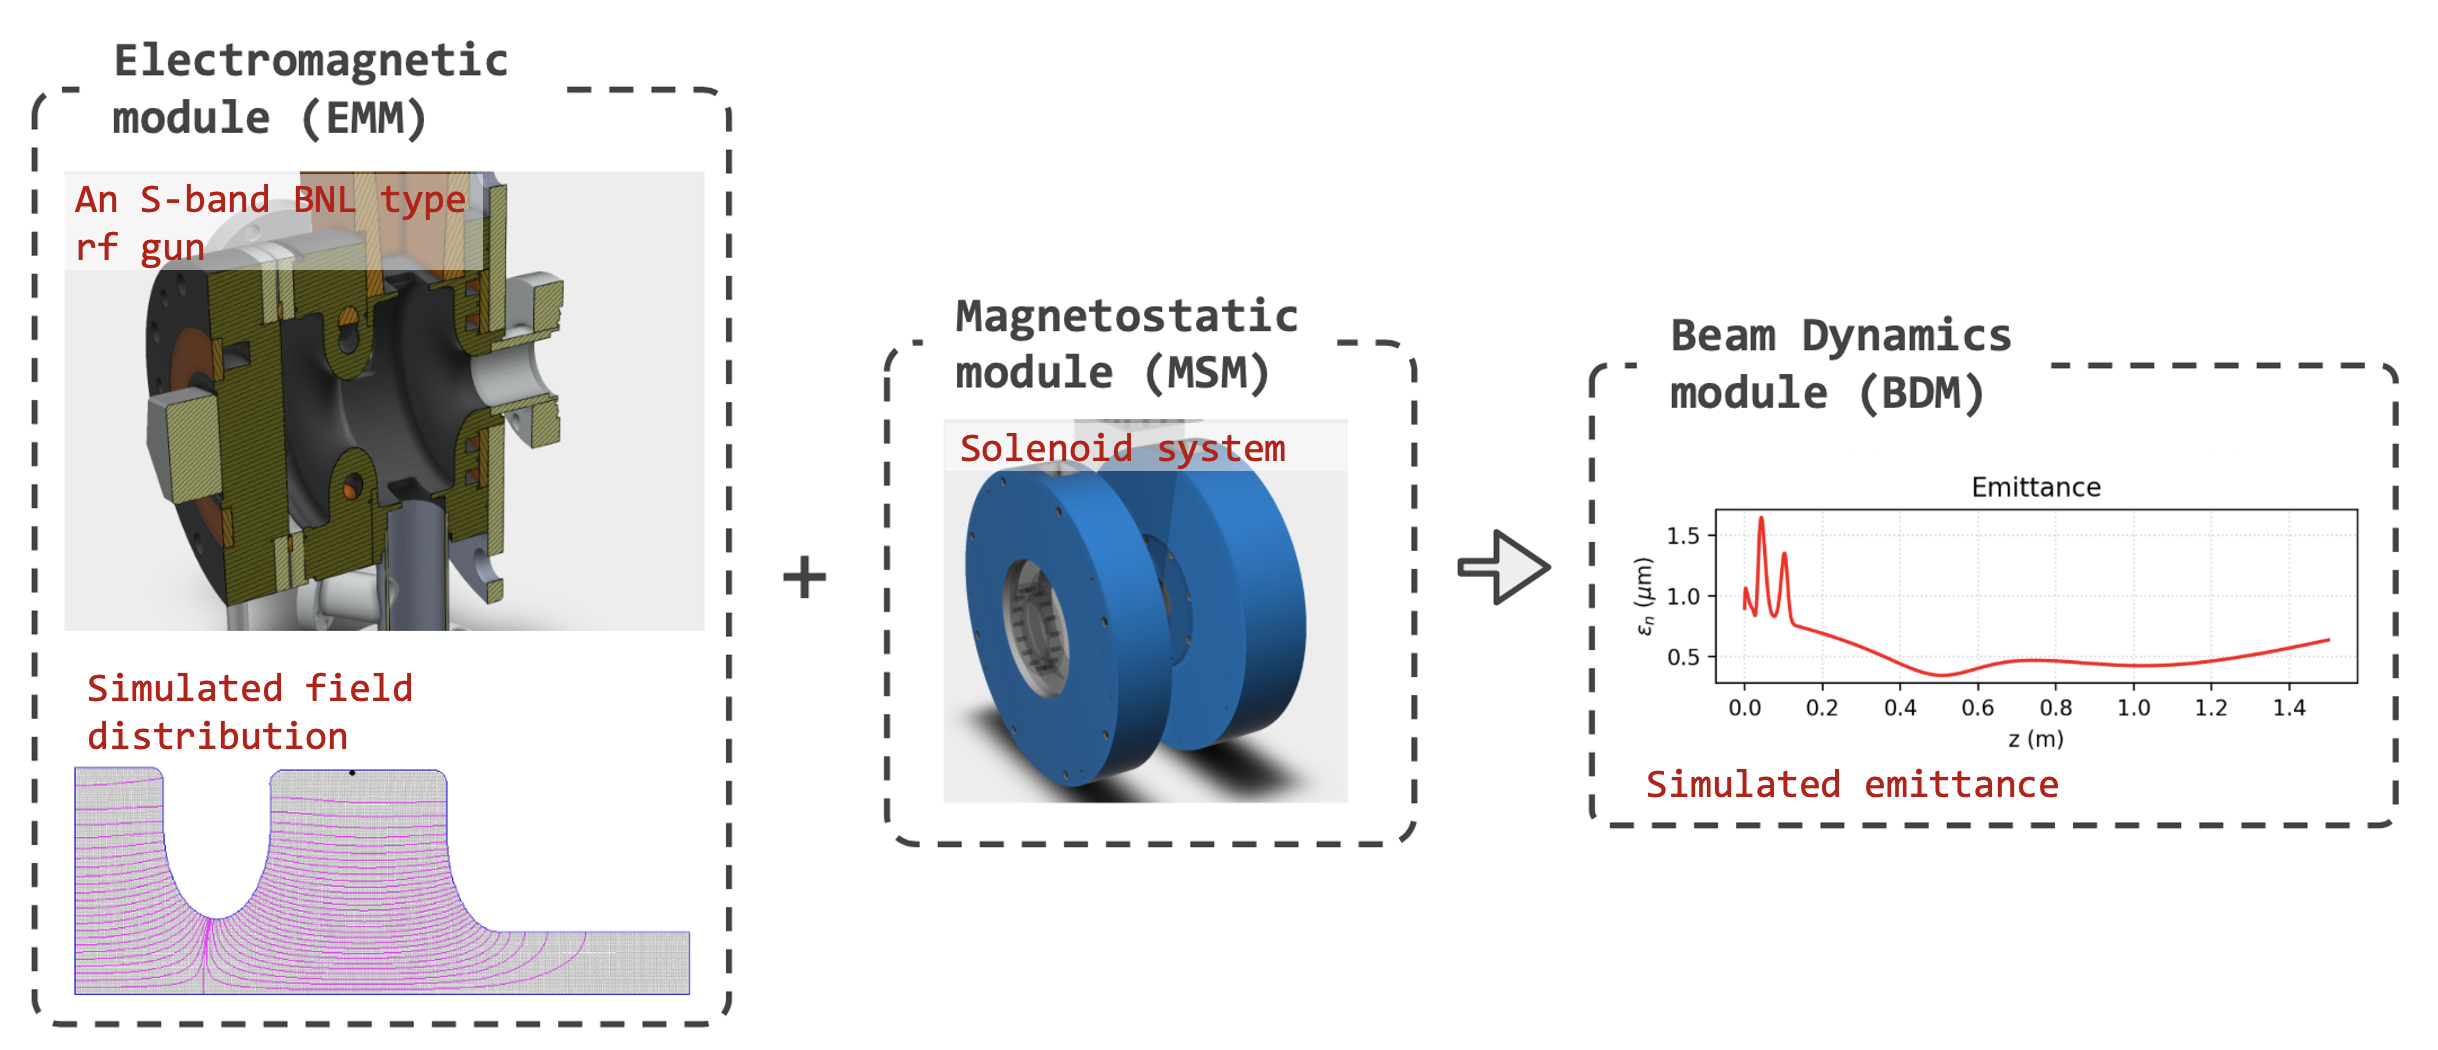
\includegraphics[width=0.4\textwidth]{../2023WSC/setup2.png}
    $\rightarrow$
    minimize sum-of-squares
\end{center}

\bigskip

\begin{center}
    minimize
    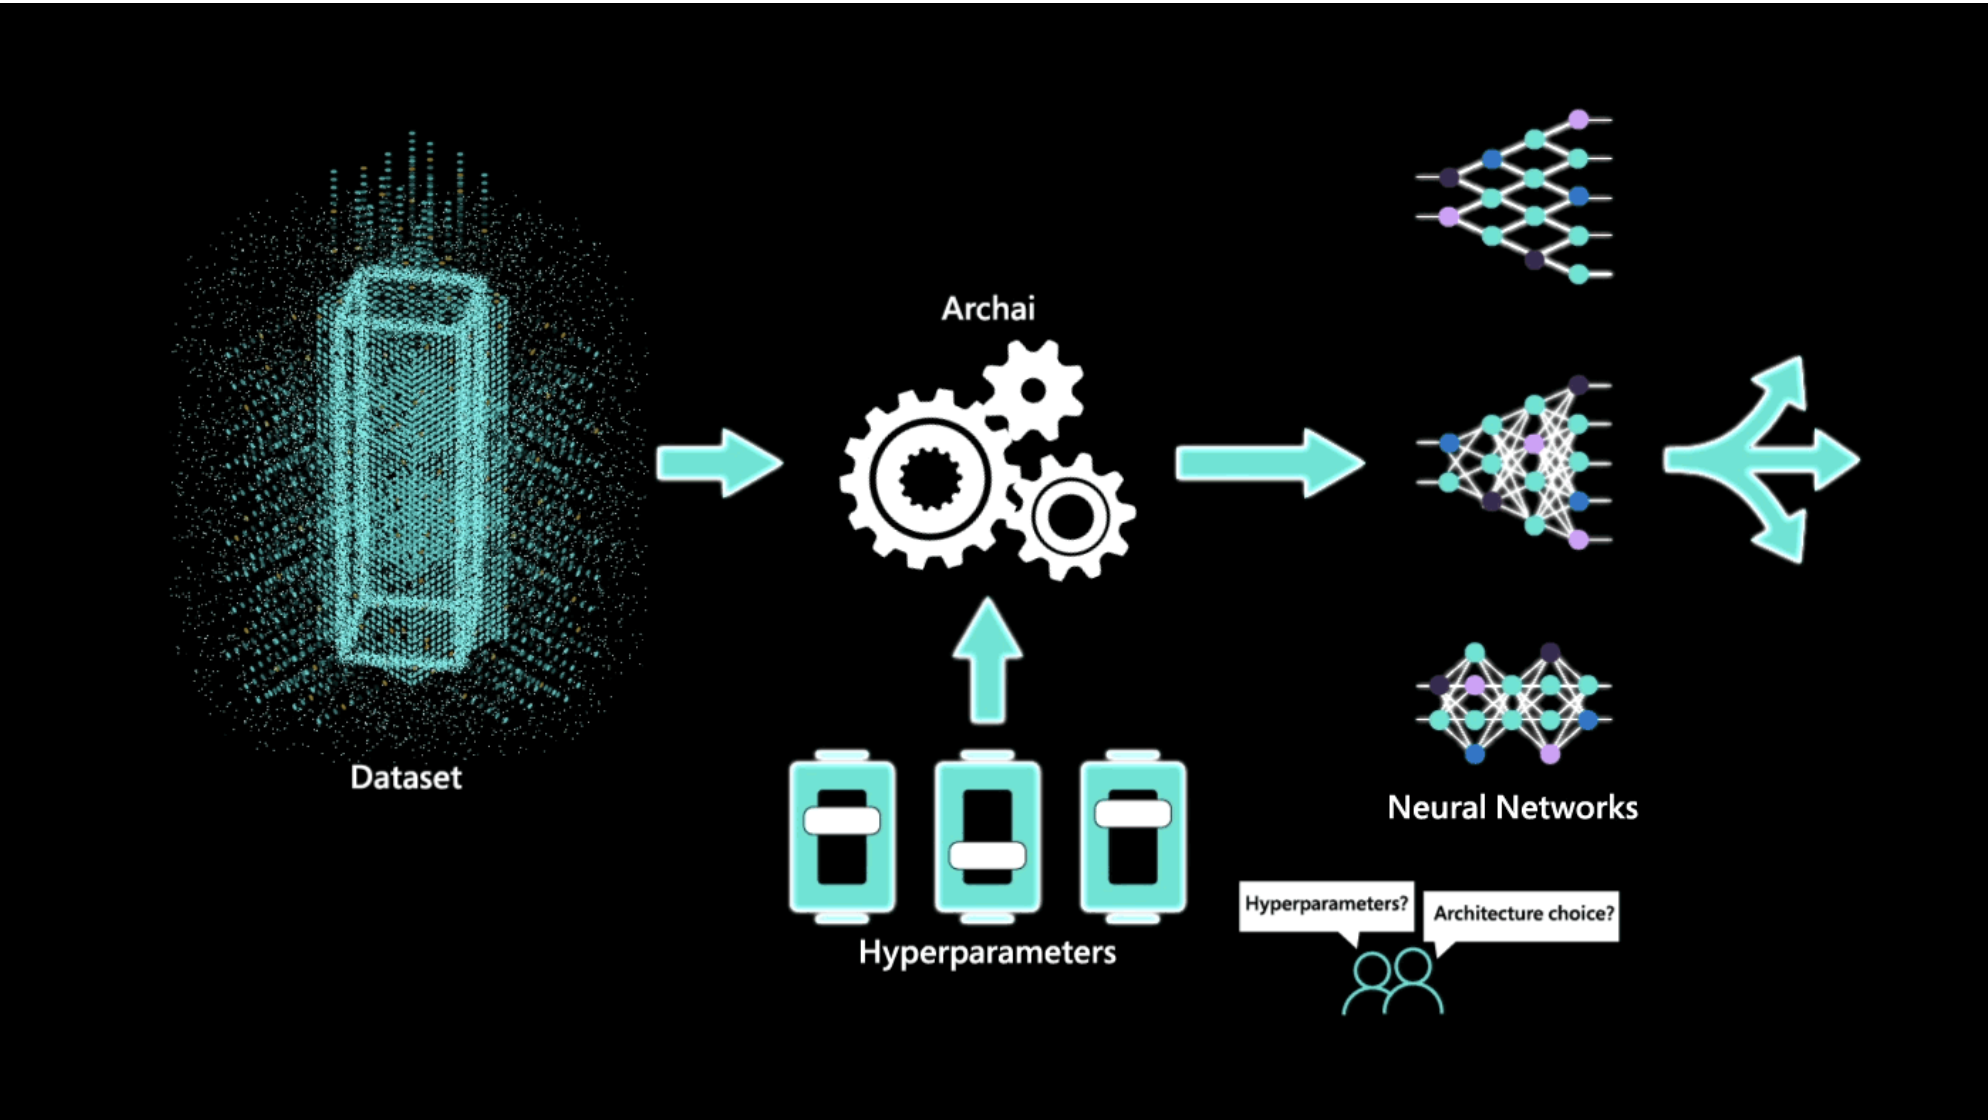
\includegraphics[width=0.4\textwidth]{../img/probs/microsoft-nas.png},
    minimize $f(x)$
\end{center}
\end{frame}

\begin{frame}\frametitle{Modeling Gray Box as Multi-Layer}
$$
\min f(x, S(x))
$$
s.t.
$$
g(x, S(x)) \leq 0
$$
where
$x$ are design variables;
$S(x)$ is an expensive ``simulation'' black-box

Then scalarization / acquisition function:

$$
\min A(f(x, S(x), w))
$$
\end{frame}

\begin{frame}\frametitle{ParMOO}
Built to manage complexity of all these layers
\begin{itemize}
 \item mainly targeting trust region methods originally
 \item often asked to compare against BO Torch, which is similar software for
 BO
 \item was looking into implementing some BO methods in ParMOO
\end{itemize}
\end{frame}

\begin{frame}\frametitle{Challenge of surrogate uncertainty}
\begin{itemize}
  \item Need to propagate uncertainty info through multiple layers
  \item BO Torch does this non intrusively via MC simulation
  \item Can we do it analytically?
\end{itemize}
\end{frame}

\begin{frame}\frametitle{Option 1: Propagate Uncertainty through nonlinear mappings}

Use a Gaussian process fed into a sum-of-squares function with expected
improvement acquisition function and any scalarization:

\begin{itemize}
  \item gaussian distribution
  \item goes into sum-of-square loss and becomes chi-squared
  \item goes into aug chebyshev and is still chi-squared above the cutoff but
  more complicated near the "0" values
\end{itemize}
\end{frame}

\begin{frame}\frametitle{Option 2: Solve a constraint optimization problem}

Use a Gaussian process fed into an algebraic function with lower confidence
bound acquisition function and augmented chebyshev scalarization:

To evaluate $f$, solve $f(x) = \min f(x, s)$ s.t. $s \in [S(x) - CB, S(x) + CB]$.

Depending on solver used, $\frac{df}{ds}$ could be approximated by the dual
solution?

\end{frame}

\begin{frame}

That's it!

Talk to me if you have thoughts on how to finish the idea!

Also (unrelated) talk to me if you are interested in solving multiobjective
optimization problems on graphs (with Siemens EDA)!

\end{frame}

\end{document}
